% =====================================================================================
% fig_agreement.tex: do the prototypes separate the classes? (Q4; Notion E8)
%
% What the experiment tests: for each prototype, the distribution of its agreement
%   (Hamming similarity on cared bits; for node prototypes, of the best-matching node of
%   each graph) over the training graphs, one histogram per class. A prototype is useful
%   if its agreement separates the classes; separation = |2 AUC - 1| of the agreement as
%   a class score.
% Plot: one row per dataset (Mutagenicity, BAMultiShapes), the prototypes cited by the
%   head (with at least one cared bit), sorted by separation; per prototype a small step
%   histogram per class, separation and cared bits in the title. (Head thresholds as
%   vertical lines: not drawn yet.)
% What it shows: which prototypes carry the decision and how cleanly; that prototypes
%   with no cared bit are constant (agreement 1 for every graph) and are hidden.
% What it does not show: what the prototype means (fig_prototypes.tex); whether the head
%   uses it alone or in combination (fig_explanation.tex); stability across folds.
% Data: agreement.{png,json,npz} written by every train_proto.py run (utils/agreement.py)
%   and by the explorer (explorer/, same computation); one chosen fold per dataset of the
%   final NMP+QAT run (say which fold, and pick it by a stated rule, e.g. median test
%   accuracy, not the best-looking one).
% GENERATED BY: python plot_paper.py agreement   (sources: configs/paper_figures.yaml, code:
%   utils/paper_figures.py, branch feat/paper-figures). "preliminary: true" in the config
%   stamps PRELIMINARY on the figure; set it to false only when every source is final.
% STATUS: PRELIMINARY version drawn 2026-10-21 (qat_nmp fold 7 on Mutagenicity, qat_nmp_3fold on BAMultiShapes, representative folds). Final after E1.
% TODO:
%   [ ] choose fold rule; plotting script -> paper/figures/fig_agreement.pdf.
%   [ ] mean-pooled agreement variant for NMP (BAMultiShapes max-agreement plot was
%       uninformative, todo P1).
% =====================================================================================
\begin{figure*}[t]
  \centering
  \IfFileExists{figures/fig_agreement_Mutagenicity.pdf}{%
    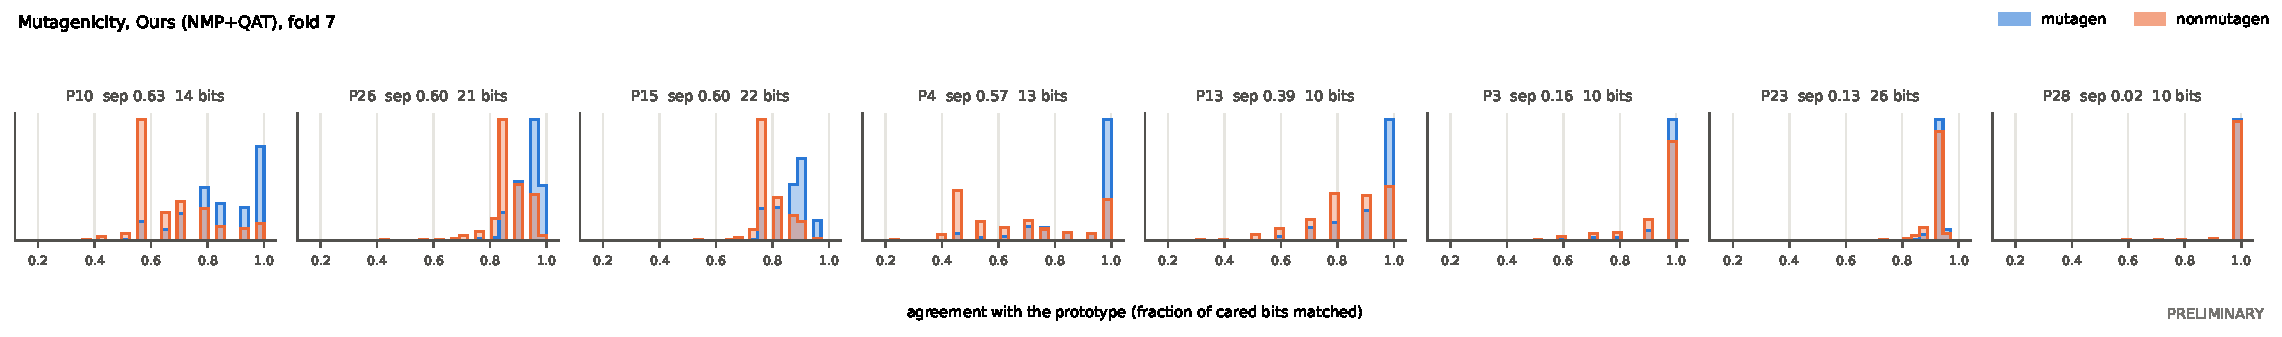
\includegraphics[width=\textwidth]{figures/fig_agreement_Mutagenicity.pdf}%
  }{\fbox{\parbox[c][3cm]{0.95\textwidth}{\centering\todo{fig\_agreement\_Mutagenicity.pdf}}}}\\[4pt]
  \IfFileExists{figures/fig_agreement_BaMultiShapes.pdf}{%
    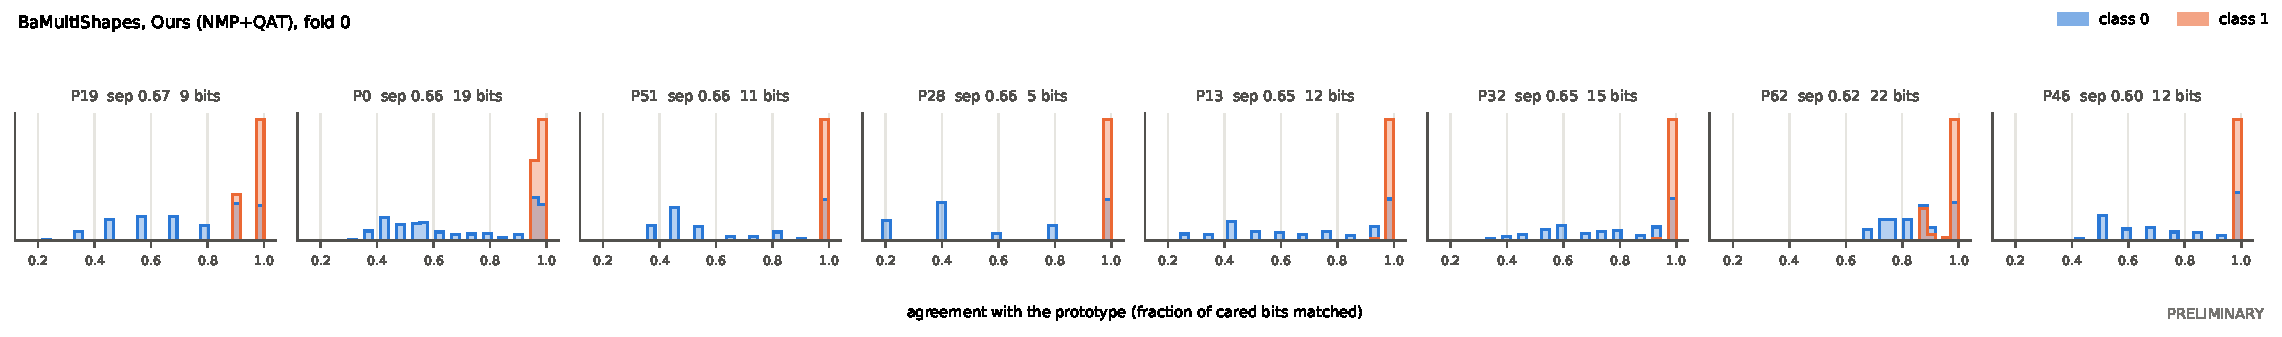
\includegraphics[width=\textwidth]{figures/fig_agreement_BaMultiShapes.pdf}%
  }{\fbox{\parbox[c][3cm]{0.95\textwidth}{\centering\todo{fig\_agreement\_BaMultiShapes.pdf}}}}\\[4pt]
  \caption{Agreement of the training graphs with each prototype cited by the explanations
    (best matching node, share of the cared bits that match), one histogram per class,
    prototypes by decreasing class separation $|2\,\mathrm{AUC}-1|$ (title, with the number
    of cared bits). Representative fold (median test balanced accuracy).}
  \label{fig:agreement}
\end{figure*}
